\documentclass{article}
\usepackage{geometry}
\usepackage{graphicx}
\renewcommand{\familydefault}{\sfdefault}
\usepackage{helvet}
\title{Assignment 1}
\author{Joe Brew}
\usepackage{Sweave}
\begin{document}
\newgeometry{margin=1.5cm}
\Sconcordance{concordance:ass1.tex:ass1.Rnw:%
1 7 1 1 0 5 1 1 6 23 1 1 8 1 3 5 1 1 8 1 3 4 1 1 8 1 3 5 1 1 8 1 3 11 1 %
1 12 1 3 4 1 1 12 1 2 2 1}

\maketitle



\section*{Note to Professor}
\addcontentsline{toc}{subsection}{Note to Professor}
Dr. Cantrell,
\\ 
Please take note of two things: \begin{enumerate}
\item I carried out this assignment using R.  This was due to my late entry to the class (Friday, 10 January) and the fact that I was not able to obtain SAS until today (Tuesday, 14 January).
\item This assignment comes approximately one week late (for the aforementioned reasons). \\
\end{enumerate}
Thank you for your understanding - I assure you that I will get on the SAS train as soon as possible.

\vspace{50mm}

\tableofcontents
\newgeometry{margin=1.5cm}

\begin{center}
\section*{Histograms, boxplots and qq-plots}
\end{center}
\addcontentsline{toc}{subsection}{Histograms, boxplots and qq-plots}

\subsection*{SYSBP}
\addcontentsline{toc}{subsection}{SYSBP}
\begin{center}
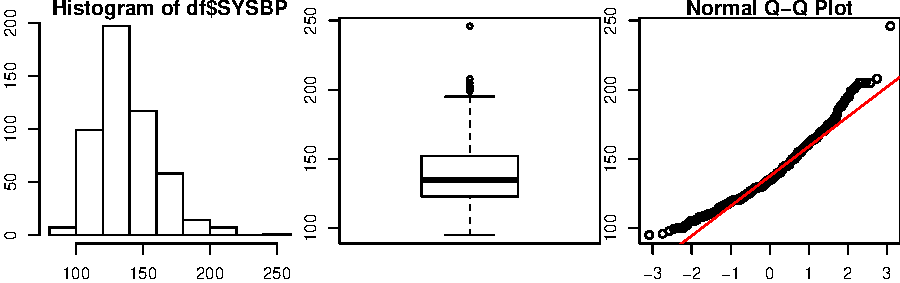
\includegraphics{ass1-002}
\end{center}


\subsection*{LNSBP}
\addcontentsline{toc}{subsection}{LNSBP}
\begin{center}
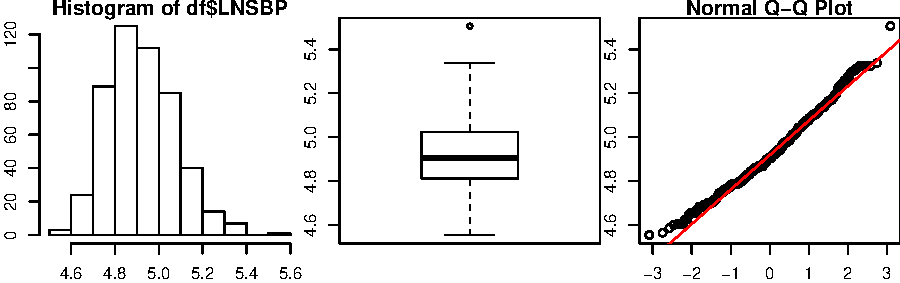
\includegraphics{ass1-003}
\end{center}

\subsection*{BMI}
\addcontentsline{toc}{subsection}{BMI}
\begin{center}
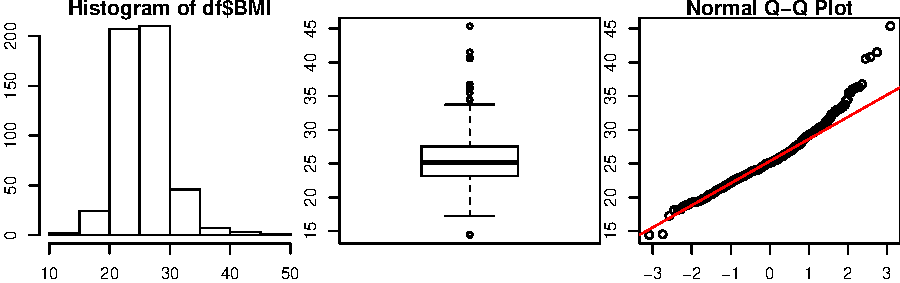
\includegraphics{ass1-004}
\end{center}


\subsection*{AGE}
\addcontentsline{toc}{subsection}{AGE}
\begin{center}
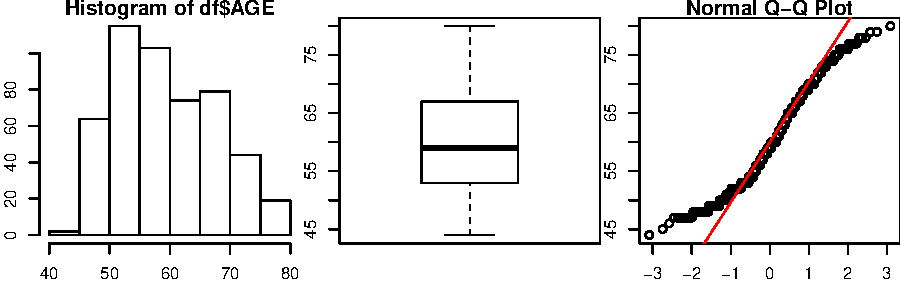
\includegraphics{ass1-005}
\end{center}

\newgeometry{margin=1.5cm}

\begin{center}
\section*{Scatterplots and LOESS curves}
\end{center}
\addcontentsline{toc}{subsection}{Scatterplots and LOESS curves}

\subsection*{Y = SYSBP, X = AGE}
\addcontentsline{toc}{subsection}{Y = SYSBP, X = AGE}
\begin{center}
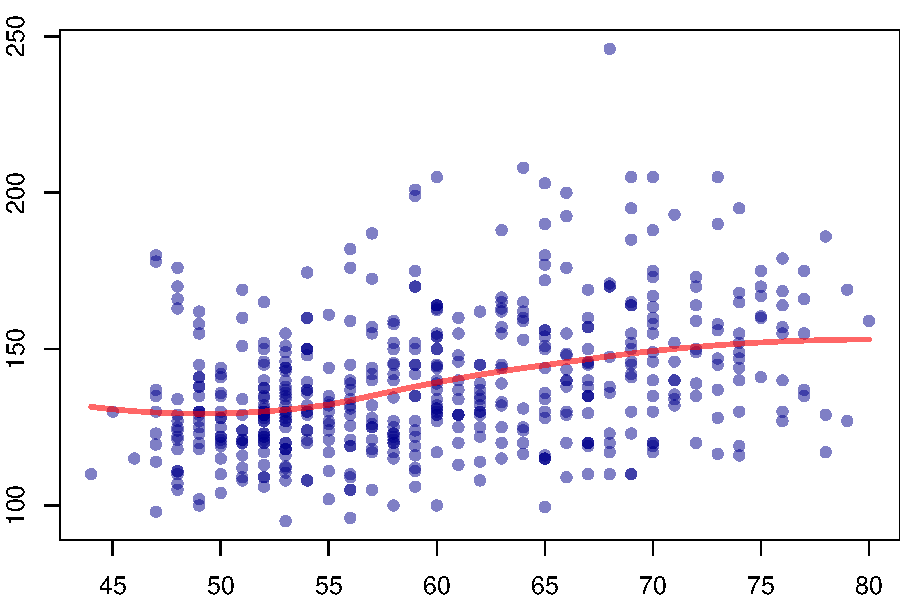
\includegraphics{ass1-006}
\end{center}

\subsection*{Y = SYSBP, X = BMI}
\addcontentsline{toc}{subsection}{Y = SYSBP, X = BMI}
\begin{center}
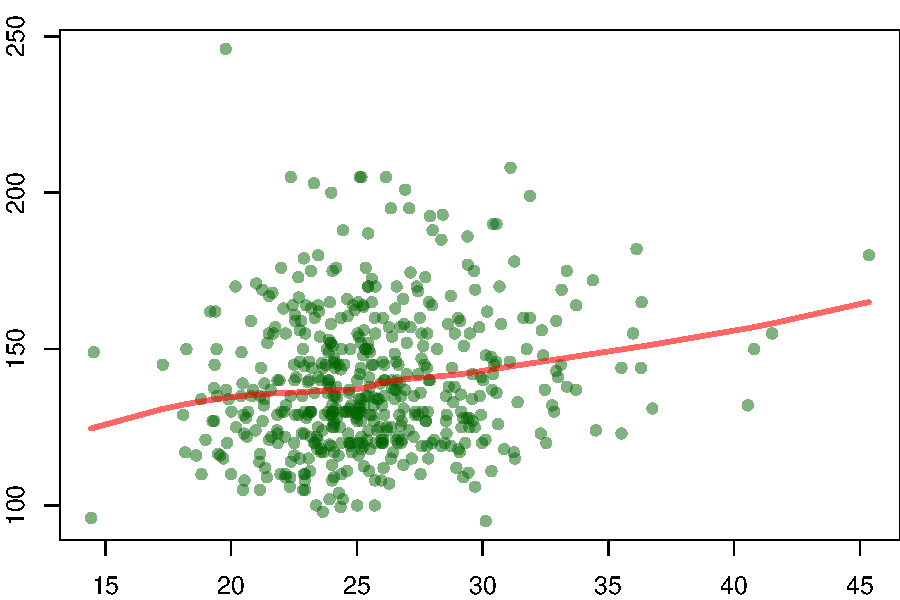
\includegraphics{ass1-007}
\end{center}
\end{document}

